\section{可行变化}
\label{sec:kkt-variations}

无约束时，最优性的论证是沿每个方向走一小步，目标都不能下降。有了约束，问题变成：站在候选点上，究竟可以朝哪些方向移动？本节先只看可行集合本身回答这个问题，再看约束函数给出的线性近似，并比较两者。这两个对象不同：前者是真实能走的方向，后者是约束函数在一阶意义下允许的方向。

\subsection{直线移动与切锥}
\label{sec:kkt-tangent-cone}

\paragraph{沿直线可行}
第~\ref{chap:optimization}章已经定义了可行方向：若$t>0$充分小时$\bar{\bm{x}}+t\bm{d}\in\bm{C}$，就称$\bm{d}$是$\bar{\bm{x}}$处的可行方向。可行集凸的时候，这个概念够用。任取$\bm{y}\in\bm{C}$，线段$\bar{\bm{x}}+t(\bm{y}-\bar{\bm{x}})$（$0\leq t\leq1$）都在$\bm{C}$里，所以每个$\bm{y}-\bar{\bm{x}}$都是可行方向，如图~\ref{fig:kkt-line-vs-arc}(a)。

\begin{BookInlineFigure}
  \centering
  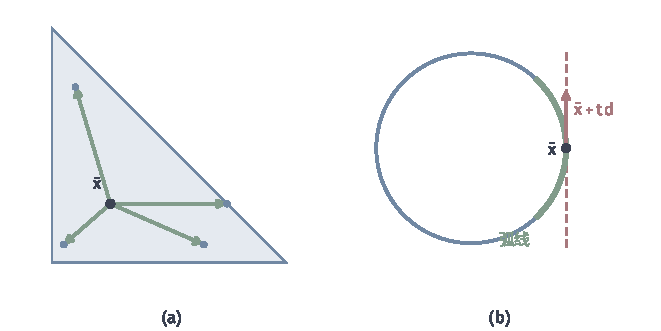
\includegraphics[width=112mm]{figures/05-optimization/06-constrained-optimization/matplotlib/kkt-line-vs-arc/figure.pdf}
  \caption{直线移动与弧线移动。(a)凸集中，从$\bar{\bm{x}}$到任意可行点的线段（绿色箭头）都留在集合内。(b)可行集是单位圆周（蓝线）。从$\bar{\bm{x}}=(1,0)$沿切线走的红色直线立刻离开圆周，而绿色弧线一直可行，并且在$\bar{\bm{x}}$处与直线相切。}
  \label{fig:kkt-line-vs-arc}
\end{BookInlineFigure}

可行集弯曲时，这个定义就不够用了。设$\bm{C}$是单位圆周，也就是$h(\bm{x})=x_1^2+x_2^2-1=0$的解集，取$\bar{\bm{x}}=(1,0)$。若$\bar{\bm{x}}+t\bm{d}$对小的$t>0$都在圆周上，展开$h$并除以$t$，得到
\[
 2d_1+t\lVert\bm{d}\rVert_2^2=0\quad\text{对所有充分小的}\ t>0.
\]
令$t$取两个不同的值，两式相减得$\lVert\bm{d}\rVert_2=0$。所以除零方向外没有可行方向。

可是点明明能沿圆周移动，图~\ref{fig:kkt-line-vs-arc}(b)的绿色弧线就是这样的移动。直线走不通，弧线走得通，弧线在出发时的速度方向是$(0,1)$。因此“能走的方向”不应理解成沿直线可行，而应理解成沿某条可行路径出发的速度。

\paragraph{用放大镜定义方向}
为了把这个想法写成定义，可以想象拿放大镜对准$\bar{\bm{x}}$看可行集。放大倍数越高，圆弧看起来越直，极限是一条直线。写成算式，就是取趋于$\bar{\bm{x}}$的可行点列，把位移除以一个趋于零的正数，看它的极限。

\begin{definition}[切锥]
\label{def:kkt-tangent-cone}
设$\bm{C}\subseteq\mathbb{R}^n$，$\bar{\bm{x}}\in\bm{C}$。称$\bm{d}\in\mathbb{R}^n$是$\bm{C}$在$\bar{\bm{x}}$处的切向量，如果存在可行点列$\bm{x}^{(k)}\in\bm{C}$与正数列$t_k$，使$\bm{x}^{(k)}\to\bar{\bm{x}}$，$t_k\downarrow0$，并且
\begin{equation}
 \frac{\bm{x}^{(k)}-\bar{\bm{x}}}{t_k}\to\bm{d}.
 \label{eq:kkt-tangent-limit}
\end{equation}
全体切向量组成的集合称为\term{切锥}（tangent cone），记为$\bm{T}_{\bm{C}}(\bar{\bm{x}})$。
\end{definition}

上标$(k)$是点列编号，不表示算法迭代。这里$1/t_k$就是放大倍数，点列可以是沿曲线取的点，也可以是在集合中跳跃着逼近的点。沿固定直线可行的方向一定是切向量：取$\bm{x}^{(k)}=\bar{\bm{x}}+t_k\bm{d}$即可。反过来不成立，圆周就是反例。

下面在圆周上走一遍定义。取$t_k=2^{-(k-1)}$，$\bm{x}^{(k)}=(\cos t_k,\sin t_k)$，放大后的位移是
\[
 \frac{\bm{x}^{(k)}-\bar{\bm{x}}}{t_k}=\Bigl(\frac{\cos t_k-1}{t_k},\frac{\sin t_k}{t_k}\Bigr).
\]
前三项依次约为$(-0.460,0.841)$、$(-0.245,0.959)$、$(-0.124,0.990)$，极限是$(0,1)$。

图~\ref{fig:kkt-tangent-sequence}左边是原始尺度下的割线，它们越来越贴近圆弧；右边是放大后的位移，绿色箭头收拢到红色的$(0,1)$。换成$t_k/s$（$s>0$）作分母，极限变成$s(0,1)$；沿圆周的另一侧取点，得到$-s(0,1)$。所以切锥至少包含整条竖直直线。下一小节会用约束函数证明切锥恰好就是这条直线。

\begin{BookInlineFigure}
  \centering
  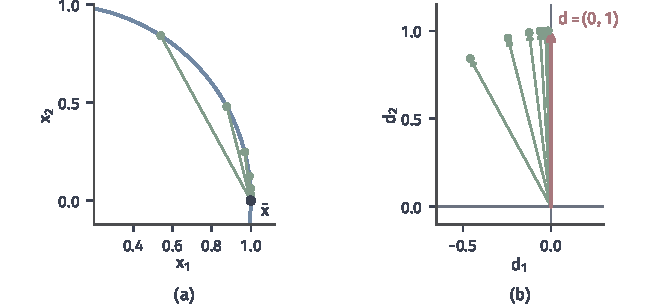
\includegraphics[width=112mm]{figures/05-optimization/06-constrained-optimization/matplotlib/kkt-tangent-sequence/figure.pdf}
  \caption{切向量是放大后位移的极限。可行集为单位圆周，$\bar{\bm{x}}=(1,0)$，$t_k=2^{-(k-1)}$（$k=1,\ldots,6$）。(a)绿点是$\bm{x}^{(k)}=(\cos t_k,\sin t_k)$，绿线是割线。(b)绿色箭头是$(\bm{x}^{(k)}-\bar{\bm{x}})/t_k$，它们趋于红色箭头$\bm{d}=(0,1)$。}
  \label{fig:kkt-tangent-sequence}
\end{BookInlineFigure}

\paragraph{切锥的基本性质}
后面的证明要用到切锥的两条性质，第二条尤其重要，它允许我们用切向量的极限产生新的切向量。

\begin{lemma}[切锥是闭锥]
\label{lem:kkt-tangent-closed}
$\bm{T}_{\bm{C}}(\bar{\bm{x}})$包含零向量，对正数倍封闭，并且是闭集。
\end{lemma}

\begin{proof}
取$\bm{x}^{(k)}=\bar{\bm{x}}$就得到零向量。若$\bm{d}$对应$(\bm{x}^{(k)},t_k)$，$s>0$，则同一点列配$t_k/s$给出$s\bm{d}$。

再证闭性。设切向量列$\bm{d}_l\to\bm{d}$。对每个$l$，由定义可以在$\bm{d}_l$对应的点列中取一项，得到可行点$\bm{y}_l$和正数$\epsilon_l<1/l$，使
\[
 \lVert\bm{y}_l-\bar{\bm{x}}\rVert_2\leq\frac1l,\qquad
 \Bigl\lVert\frac{\bm{y}_l-\bar{\bm{x}}}{\epsilon_l}-\bm{d}_l\Bigr\rVert_2\leq\frac1l.
\]
令$l\to\infty$，有$\bm{y}_l\to\bar{\bm{x}}$，$\epsilon_l\to0$（必要时取子列使$\epsilon_l$单调递减），位移比趋于$\bm{d}$。所以$\bm{d}$是切向量。
\end{proof}

图~\ref{fig:kkt-tangent-cones}是几种常见的形状。内点处四周都能走，切锥是全空间。光滑边界上，放大后边界变成直线，切锥是半空间。角点处切锥是楔形。尖点处两条边界相切，放大后楔形被压成一条线，切锥只剩一条射线。

\begin{BookInlineFigure}
  \centering
  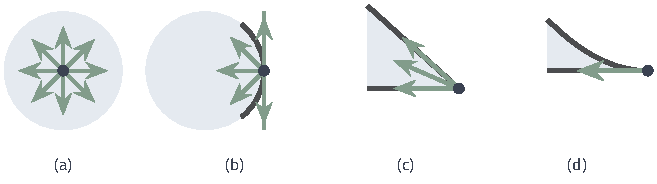
\includegraphics[width=111.3mm]{figures/05-optimization/06-constrained-optimization/tikz/kkt-tangent-cones/figure.pdf}
  \caption{切锥的四种形状。浅蓝区域是可行集，黑点是基点，绿色箭头表示切向量，深灰粗线是边界。(a)内点：全部方向。(b)光滑边界：半空间，边界上的绿线是它的分界。(c)角点：楔形。(d)尖点：只有一条射线。}
  \label{fig:kkt-tangent-cones}
\end{BookInlineFigure}

切锥未必是凸集。集合$\{\bm{x}:x_1x_2=0\}$由两条坐标轴组成，它在原点的切锥就是这两条坐标轴本身。名字里的“锥”只表示对正数倍封闭。

\subsection{一阶必要条件}
\label{sec:kkt-first-order}

现在可以回答：局部最小点在切向量上要满足什么？直观上，沿任何可行路径出发，目标都不能以一阶速度下降。把路径换成切锥定义中的点列，证明只需要一次Taylor展开。

\begin{theorem}[切锥上的一阶必要条件]
\label{thm:kkt-tangent-necessary}
设$\bm{x}^\star$是$f$在$\bm{C}$上的局部最小点，$f$在$\bm{x}^\star$处可微。则
\begin{equation}
 \langle\nabla f(\bm{x}^\star),\bm{d}\rangle\geq0\quad\text{对所有}\ \bm{d}\in\bm{T}_{\bm{C}}(\bm{x}^\star).
 \label{eq:kkt-tangent-necessary}
\end{equation}
\end{theorem}

\begin{proof}
取切向量$\bm{d}$及相应的$\bm{x}^{(k)}$、$t_k$，记位移$\bm{u}_k=\bm{x}^{(k)}-\bm{x}^\star$。$f$在$\bm{x}^\star$处可微，所以
\[
 f(\bm{x}^{(k)})-f(\bm{x}^\star)=\langle\nabla f(\bm{x}^\star),\bm{u}_k\rangle+r_k,
 \qquad\frac{r_k}{\lVert\bm{u}_k\rVert_2}\to0,
\]
其中$\bm{u}_k=\bm{0}$时取$r_k=0$，比值按零理解。

$k$充分大时$\bm{x}^{(k)}$落在式~\eqref{eq:kkt-local-min}的邻域内，左端非负。两边除以$t_k$，得到
\[
 0\leq\Bigl\langle\nabla f(\bm{x}^\star),\frac{\bm{u}_k}{t_k}\Bigr\rangle+\frac{r_k}{t_k}.
\]

由$\bm{u}_k/t_k\to\bm{d}$知$\lVert\bm{u}_k\rVert_2/t_k$有界，所以$r_k/t_k\to0$。令$k\to\infty$，即得式~\eqref{eq:kkt-tangent-necessary}。
\end{proof}

在预算例上试用这个条件（$\tau=2$）。先看不是最优的点$\bar{\bm{x}}=(1,1)$，它在预算线上，梯度是$(-1,0)$。沿预算线的切向量$\bm{d}=(1,-1)$有
\[
 \langle\nabla f(\bar{\bm{x}}),\bm{d}\rangle=-1<0.
\]
直接代入也一样：$f(1+s,1-s)=\frac12[(1-s)^2+s^2]$在$s=0$处的导数是$-1$。所以$(1,1)$不是局部最小点。

再看$\bm{x}^\star=(3/2,1/2)$。这里切锥是半平面$\{\bm{d}:d_1+d_2\leq0\}$，梯度是$(-1/2,-1/2)$，于是对切锥中每个$\bm{d}$，
\[
 \langle\nabla f(\bm{x}^\star),\bm{d}\rangle=-\frac12(d_1+d_2)\geq0.
\]
必要条件成立。图~\ref{fig:kkt-first-order-test}比较了这两个点：(a)中负梯度有沿边界的分量，绿色切向量与负梯度成锐角；(b)中负梯度与边界垂直，沿边界两侧移动都没有一阶下降。

\begin{BookInlineFigure}
  \centering
  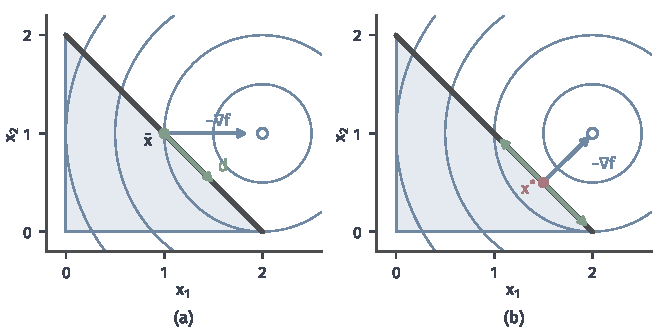
\includegraphics[width=112mm]{figures/05-optimization/06-constrained-optimization/matplotlib/kkt-first-order-test/figure.pdf}
  \caption{切向量上的一阶检验（预算例，$\tau=2$）。空心点是理想分配$\bm{c}$，蓝色箭头是负梯度，绿色箭头是沿预算线的切向量。(a)在$\bar{\bm{x}}=(1,1)$，切向量$\bm{d}=(1,-1)$与负梯度成锐角，目标可以下降。(b)在红点$\bm{x}^\star=(3/2,1/2)$，负梯度垂直于预算线，不存在下降的切向量。}
  \label{fig:kkt-first-order-test}
\end{BookInlineFigure}

\paragraph{凸可行集：法锥}
可行集凸时，每个$\bm{y}-\bm{x}^\star$都是切向量，所以条件可以写成对全部可行点的检验，把切向量这个中间概念拿掉。我们把这个条件从“梯度与所有可行方向的夹角”改写到集合一侧，定义所有“指向集合外”的向量。

\begin{definition}[法锥]
\label{def:kkt-normal-cone}
设$\bm{C}\subseteq\mathbb{R}^n$是凸集，$\bar{\bm{x}}\in\bm{C}$。集合
\begin{equation}
 \bm{N}_{\bm{C}}(\bar{\bm{x}})=\{\bm{v}\in\mathbb{R}^n:\langle\bm{v},\bm{y}-\bar{\bm{x}}\rangle\leq0\ \text{对所有}\ \bm{y}\in\bm{C}\}
 \label{eq:kkt-normal-cone}
\end{equation}
称为$\bm{C}$在$\bar{\bm{x}}$处的\term{法锥}（normal cone）。
\end{definition}

法锥里的向量与所有从$\bar{\bm{x}}$出发的可行弦成钝角或直角，它们都指向集合外侧。负梯度只要落在法锥里，朝可行集内部就没有一阶下降。

\begin{theorem}[凸可行集上的一阶条件]
\label{thm:kkt-convex-set-first-order}
设$\bm{C}$是凸集，$f$在包含$\bm{C}$的开集上可微，$\bm{x}^\star\in\bm{C}$。若$\bm{x}^\star$是$f$在$\bm{C}$上的局部最小点，则
\begin{equation}
 \langle\nabla f(\bm{x}^\star),\bm{y}-\bm{x}^\star\rangle\geq0\quad\text{对所有}\ \bm{y}\in\bm{C},
 \label{eq:kkt-vi}
\end{equation}
等价地，$-\nabla f(\bm{x}^\star)\in\bm{N}_{\bm{C}}(\bm{x}^\star)$。若$f$还在$\bm{C}$上凸，则式~\eqref{eq:kkt-vi}也推出$\bm{x}^\star$是全局最小点。
\end{theorem}

\begin{proof}
必要性：$\bm{y}-\bm{x}^\star$是可行方向，也是切向量，由定理~\ref{thm:kkt-tangent-necessary}得到式~\eqref{eq:kkt-vi}。等价写法只是把$\bm{v}=-\nabla f(\bm{x}^\star)$代入式~\eqref{eq:kkt-normal-cone}。

充分性：取$\bm{y}\in\bm{C}$，$t\in(0,1]$。由$f$的凸性，
\[
 f\bigl(\bm{x}^\star+t(\bm{y}-\bm{x}^\star)\bigr)\leq(1-t)f(\bm{x}^\star)+tf(\bm{y}).
\]
移项，除以$t$，再令$t\downarrow0$，左端的差商趋于方向导数，于是
\[
 \langle\nabla f(\bm{x}^\star),\bm{y}-\bm{x}^\star\rangle\leq f(\bm{y})-f(\bm{x}^\star).
\]
由式~\eqref{eq:kkt-vi}，左端非负，所以$f(\bm{y})\geq f(\bm{x}^\star)$。
\end{proof}

式~\eqref{eq:kkt-vi}称为\term{变分不等式}（variational inequality）。图~\ref{fig:kkt-normal-cones}让预算$\tau$从大变小，法锥依次是三种形状。

$\tau=4$时最优点$\bm{c}=(2,1)$在内部，法锥只有零向量，条件退化为$\nabla f=\bm{0}$。$\tau=2$时最优点在预算线上，法锥是外法向$(1,1)$方向的射线，$-\nabla f=(1/2,1/2)$落在上面。

$\tau=1/2$时，最优点是角点$(1/2,0)$。法锥由两条边的外法向$(1,1)$、$(0,-1)$张成。这一点可以直接核对：设$\bm{v}\in\bm{N}_{\bm{C}}$，用沿两条边的可行弦方向$(-1,1)$与$(-1,0)$代入式~\eqref{eq:kkt-normal-cone}，得到$v_2\leq v_1$与$v_1\geq0$，这恰好说明
\[
 \bm{v}=v_1(1,1)+(v_1-v_2)(0,-1),\qquad v_1\geq0,\ v_1-v_2\geq0.
\]
角点的法锥比边上的法锥大，能接住更多方向的负梯度。

\begin{BookInlineFigure}
  \centering
  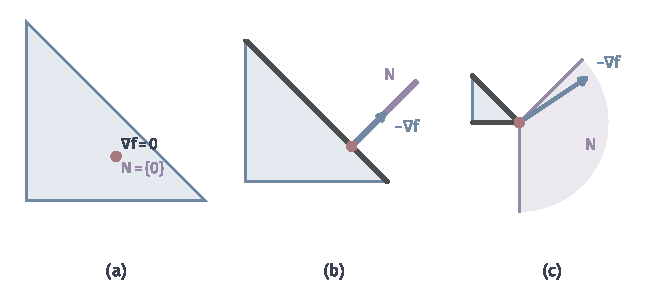
\includegraphics[width=112mm]{figures/05-optimization/06-constrained-optimization/matplotlib/kkt-normal-cones/figure.pdf}
  \caption{预算例中最优点处的法锥（紫色）。红点是最优点，蓝色箭头是负梯度（(c)中按$0.5$倍缩短）。(a)$\tau=4$，最优点在内部，法锥为$\{\bm{0}\}$。(b)$\tau=2$，法锥是一条射线，负梯度落在上面。(c)$\tau=1/2$，最优点是角点，法锥是两条外法向张成的楔形，负梯度落在其中。}
  \label{fig:kkt-normal-cones}
\end{BookInlineFigure}

定理的充分性同时需要可行集与目标都凸。只有目标凸是不够的：在单位圆周上最小化$\frac12\lVert\bm{x}-(2,0)\rVert_2^2$，点$(-1,0)$的梯度是$(-3,0)$，切向量只有$(0,s)$，与梯度垂直，一阶条件成立；可它是圆周上离$(2,0)$最远的点。本章后面还会回到这个例子。

\subsection{约束的线性化}
\label{sec:kkt-linearized}

切锥描述得准，却不好算，我们无法枚举所有点列。约束以函数形式给出时，有一个自然的替代品：在基点把约束函数展开到一阶，看一阶近似允许哪些方向。

设$\bar{\bm{x}}$可行，沿$\bm{d}$走一小步，约束函数近似变化为
\[
 g_i(\bar{\bm{x}}+t\bm{d})\approx g_i(\bar{\bm{x}})+t\langle\nabla g_i(\bar{\bm{x}}),\bm{d}\rangle.
\]
不活动的约束有余量，一阶近似不构成限制。活动约束要求这一项不为正，等式约束要求它等于零。

\begin{definition}[线性化锥]
\label{def:kkt-linearized-cone}
设$\bar{\bm{x}}\in\bm{C}$，约束函数在$\bar{\bm{x}}$处可微。集合
\begin{equation}
 \bm{F}(\bar{\bm{x}})=\left\{\bm{d}\in\mathbb{R}^n:
 \begin{aligned}
  &\langle\nabla h_j(\bar{\bm{x}}),\bm{d}\rangle=0,\ j=1,\ldots,p,\\
  &\langle\nabla g_i(\bar{\bm{x}}),\bm{d}\rangle\leq0,\ i\in A(\bar{\bm{x}})
 \end{aligned}
 \right\}
 \label{eq:kkt-linearized-cone}
\end{equation}
称为$\bar{\bm{x}}$处的\term{线性化锥}（linearized cone）。
\end{definition}

$\bm{F}(\bar{\bm{x}})$是有限个线性不等式的解集，一眼就能写出。例如预算例$\tau=1/2$的角点$(1/2,0)$处，$g_1$和$g_3$活动，于是
\[
 \bm{F}=\{\bm{d}:d_1+d_2\leq0,\ -d_2\leq0\}.
\]
单位圆周在$(1,0)$处，$\nabla h=(2,0)$，于是$\bm{F}=\{\bm{d}:d_1=0\}$，正是前面算出的竖直直线。

真实能走的方向一定通过这个一阶检查，因此切锥总在线性化锥之内。

\begin{theorem}[切锥包含于线性化锥]
\label{thm:kkt-tangent-in-linearized}
设$\bar{\bm{x}}\in\bm{C}$，$g_i$（$i\in A(\bar{\bm{x}})$）与$h_j$在$\bar{\bm{x}}$处可微。则
\begin{equation}
 \bm{T}_{\bm{C}}(\bar{\bm{x}})\subseteq\bm{F}(\bar{\bm{x}}).
 \label{eq:kkt-tangent-in-linearized}
\end{equation}
\end{theorem}

\begin{proof}
取切向量$\bm{d}$及相应的$\bm{x}^{(k)}$、$t_k$，对活动的$g_i$，由可微性，
\[
 g_i(\bm{x}^{(k)})=g_i(\bar{\bm{x}})+\langle\nabla g_i(\bar{\bm{x}}),\bm{x}^{(k)}-\bar{\bm{x}}\rangle+o(\lVert\bm{x}^{(k)}-\bar{\bm{x}}\rVert_2).
\]
这里$g_i(\bar{\bm{x}})=0$，$g_i(\bm{x}^{(k)})\leq0$。除以$t_k$并令$k\to\infty$，余项如定理~\ref{thm:kkt-tangent-necessary}的证明一样趋于零，得到
\[
 \langle\nabla g_i(\bar{\bm{x}}),\bm{d}\rangle\leq0.
\]

对$h_j$同样展开，此时左端恒为零，极限给出$\langle\nabla h_j(\bar{\bm{x}}),\bm{d}\rangle=0$。
\end{proof}

圆周的例子到这里算完了：切锥包含竖直直线，又包含于$\bm{F}=\{\bm{d}:d_1=0\}$，所以它就是这条直线。

式~\eqref{eq:kkt-tangent-in-linearized}可以是严格包含。考虑一维约束$g(x)=x^2\leq0$，可行集只有原点，切锥是$\{0\}$。可是$g'(0)=0$，线性化没有施加任何限制，$\bm{F}(0)=\mathbb{R}$。一阶近似把这条弯曲的约束看成了常值零，图~\ref{fig:kkt-linearization}(b)的黄色线就是这个近似。

\begin{BookInlineFigure}
  \centering
  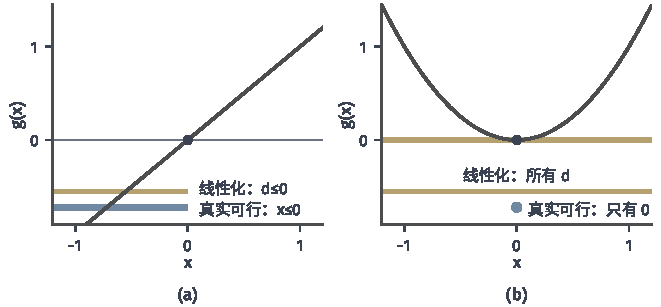
\includegraphics[width=112mm]{figures/05-optimization/06-constrained-optimization/matplotlib/kkt-linearization/figure.pdf}
  \caption{线性化与真实可行集的比较。深灰曲线是$g$，下方黄带是线性化允许的方向，蓝带（点）是真实的可行点。(a)$g(x)=x$，线性化与真实情况一致。(b)$g(x)=x^2$，$g'(0)=0$，切线（黄色）恒为零，线性化允许所有方向，而可行集只有原点。}
  \label{fig:kkt-linearization}
\end{BookInlineFigure}

二维的例子能看得更清楚。取$g_1(\bm{x})=x_2-(1-x_1)^3\leq0$，$g_2(\bm{x})=-x_2\leq0$，点$\bar{\bm{x}}=(1,0)$，两条约束都活动。可行点要满足$0\leq x_2\leq(1-x_1)^3$，所以$x_1\leq1$，可行集在$\bar{\bm{x}}$处形成一个向右的尖点。

梯度分别是$(0,1)$和$(0,-1)$，线性化要求$d_2\leq0$且$-d_2\leq0$，即$d_2=0$，于是
\[
 \bm{F}(\bar{\bm{x}})=\{\bm{d}:d_2=0\},\qquad
 \bm{T}_{\bm{C}}(\bar{\bm{x}})=\{(-s,0):s\geq0\}.
\]
线性化多出了向右的半条直线。图~\ref{fig:kkt-cusp}中的红色箭头就是虚假方向：若最小化$f(\bm{x})=-x_1$，$\bar{\bm{x}}$是全局最小点，而$\bm{d}=(1,0)$在线性化下“可行”，并使$\langle\nabla f,\bm{d}\rangle=-1<0$。只看线性化，就会误以为还能下降。

\begin{BookInlineFigure}
  \centering
  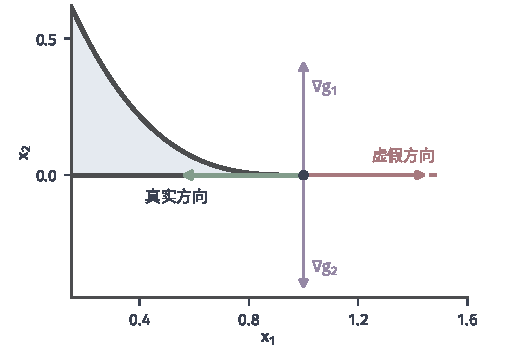
\includegraphics[width=88mm]{figures/05-optimization/06-constrained-optimization/matplotlib/kkt-cusp/figure.pdf}
  \caption{尖点处线性化引入虚假方向。浅蓝区域是可行集$0\leq x_2\leq(1-x_1)^3$，紫色箭头是两条活动约束的梯度$(0,\pm1)$。线性化只要求$d_2=0$，向左的绿色箭头是真实切向量，向右的红色箭头是虚假方向。}
  \label{fig:kkt-cusp}
\end{BookInlineFigure}

表~\ref{tab:kkt-tangent-vs-linearized}对比这两个对象。下一节要回答的问题由此而来：什么时候两者相等，使我们可以用好算的线性化锥代替真实的切锥？

\begin{BookInlineTable}
  \centering
  \begin{tabular}{@{}lll@{}}
    \toprule
    对比项 & 切锥$\bm{T}_{\bm{C}}$ & 线性化锥$\bm{F}$\\
    \midrule
    依赖什么 & 只依赖集合$\bm{C}$ & 依赖约束函数的写法\\
    含义 & 真实可行变化 & 一阶模型允许的变化\\
    计算 & 一般需要分析点列 & 解线性不等式\\
    关系 & 总包含在$\bm{F}$内 & 可能多出虚假方向\\
    \bottomrule
  \end{tabular}
  \caption{切锥与线性化锥的比较。}
  \label{tab:kkt-tangent-vs-linearized}
\end{BookInlineTable}
